\section{Tools}

To perform data analysis, we will utilize the following tools:

\begin{itemize}
    \item Python
    \item Databricks
    \item Apache Spark
    \item MSSQL
    \item Pandas
    \item Astrup Fearnleys Code Emission Calculator API
\end{itemize}

\subsection{Databricks}

Databricks is a leading platform for big data analysis, specifically designed to handle \newline large-scale datasets efficiently and effectively.
Leveraging Apache Spark as its core engine, Databricks provides a distributed computing framework that enables processing massive volumes of data in parallel across multiple nodes.
This distributed architecture allows for significant performance improvements, reducing the time it takes to process and analyze big data compared to traditional approaches.
With its ability to handle both batch and real-time data processing, Databricks empowers data engineers and analysts to extract valuable insights from vast datasets, enabling them to make data-driven decisions at scale.

One of the key advantages of using Databricks for big data analysis is its ease of use and collaborative features.
The platform offers interactive notebooks (Figure \ref{databricks_notebook})  that allow data professionals to write, execute, and share code seamlessly.
This enables collaborative data exploration and simplifies the iterative process of data analysis and model development.
Moreover, Databricks provides a rich set of built-in libraries and integrations with popular big data tools and machine learning frameworks, streamlining the development and deployment of complex data pipelines and advanced analytical models.
By abstracting the complexities of distributed data processing, Databricks empowers data teams to focus on the analysis and interpretation of results, accelerating the time-to-insight for big data projects and ultimately driving business growth and innovation.
One of the key benefits of using Databricks for big data analysis is its ability to handle large volumes of data with ease.
Whether you're working with terabytes, petabytes, or even exabytes of data, Databricks can scale to meet your needs without sacrificing performance or reliability.
This makes it an ideal solution for organizations looking to perform complex big data analysis tasks, such as machine learning, data warehousing, and real-time streaming analytics \autocite{databricksDataLakehouse}.

\begin{figure}[ht]
    \centering
    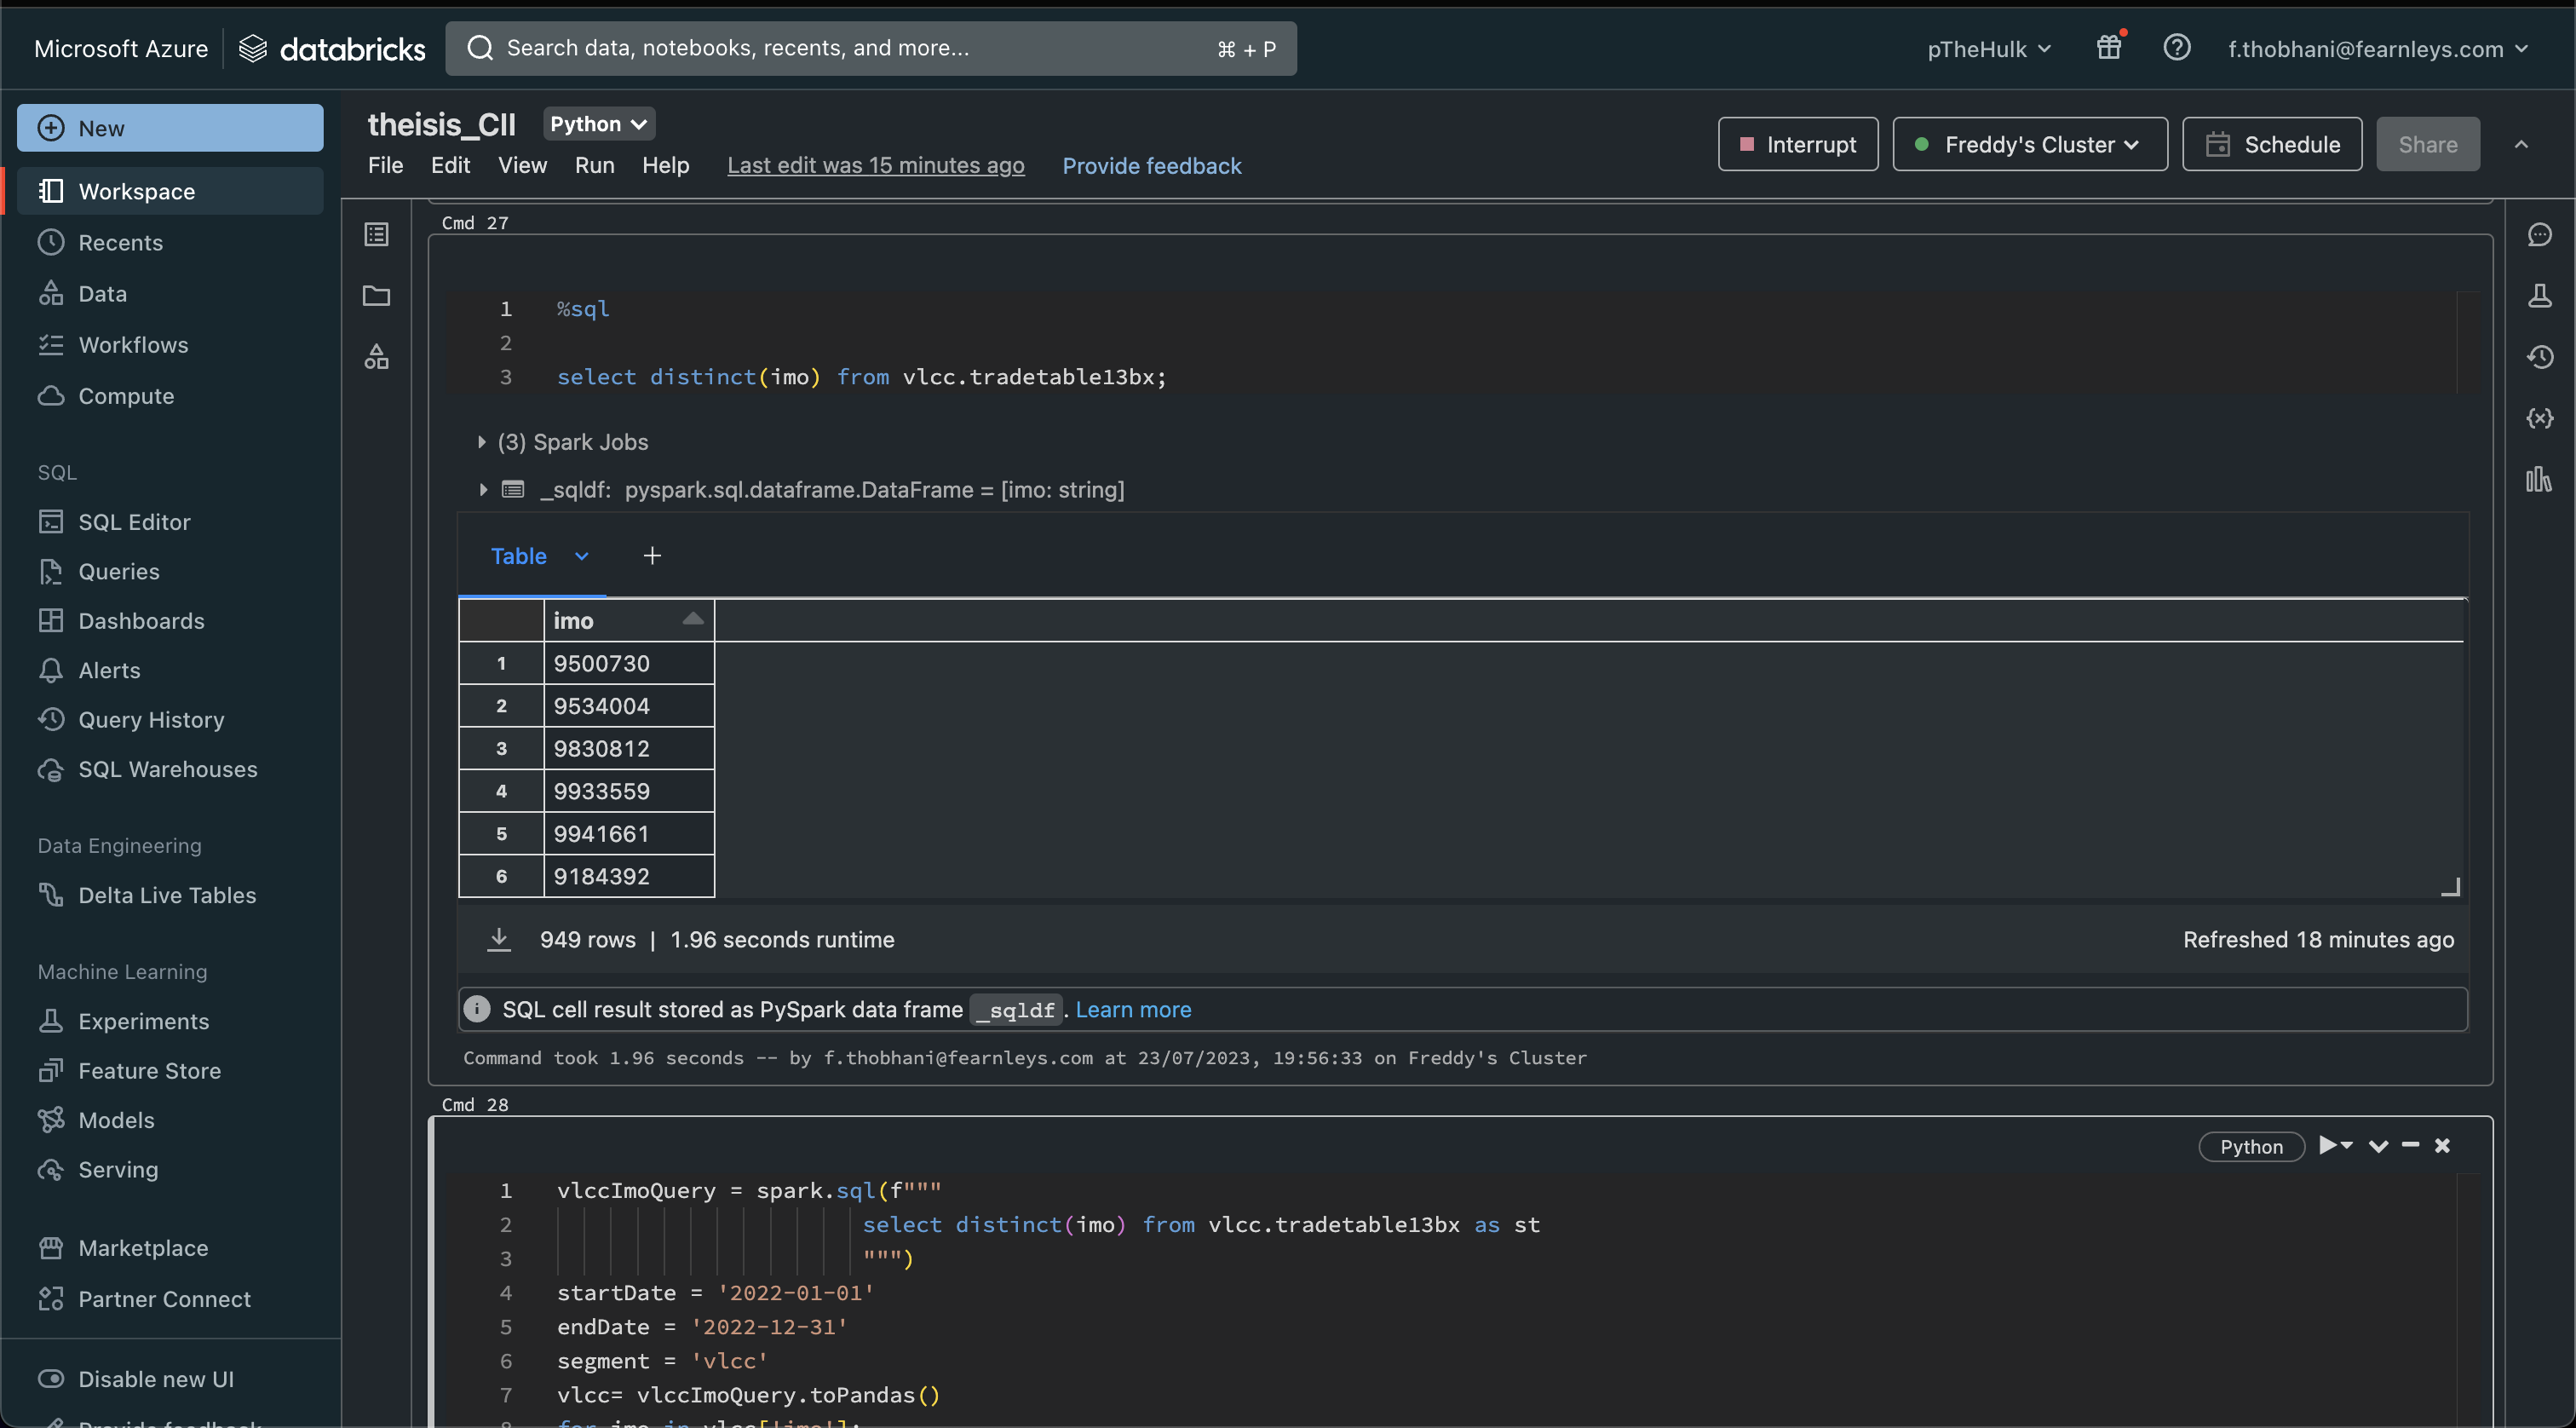
\includegraphics[width=1\textwidth]{images/databricks_notebook.png}
    \caption{Databricks Notebook}
    \label{databricks_notebook}
\end{figure}

Overall, Databricks is a highly capable platform for big data analysis that is well-suited to a wide range of use cases, from simple data processing tasks to complex machine learning and statistical analysis.

The entire analysis will be conducted on Databricks with the following configuration:

\begin{itemize}
    \item Databricks Runtime Version: 11.3 LTS (includes Apache Spark 3.3.0, Scala 2.12)
    \item 8GB Memory, 4 Cores with 1 driver and 1 worker node.
    \item Python 3
    \item Elastic Disk
\end{itemize}

\begin{figure}[ht]
    \centering
    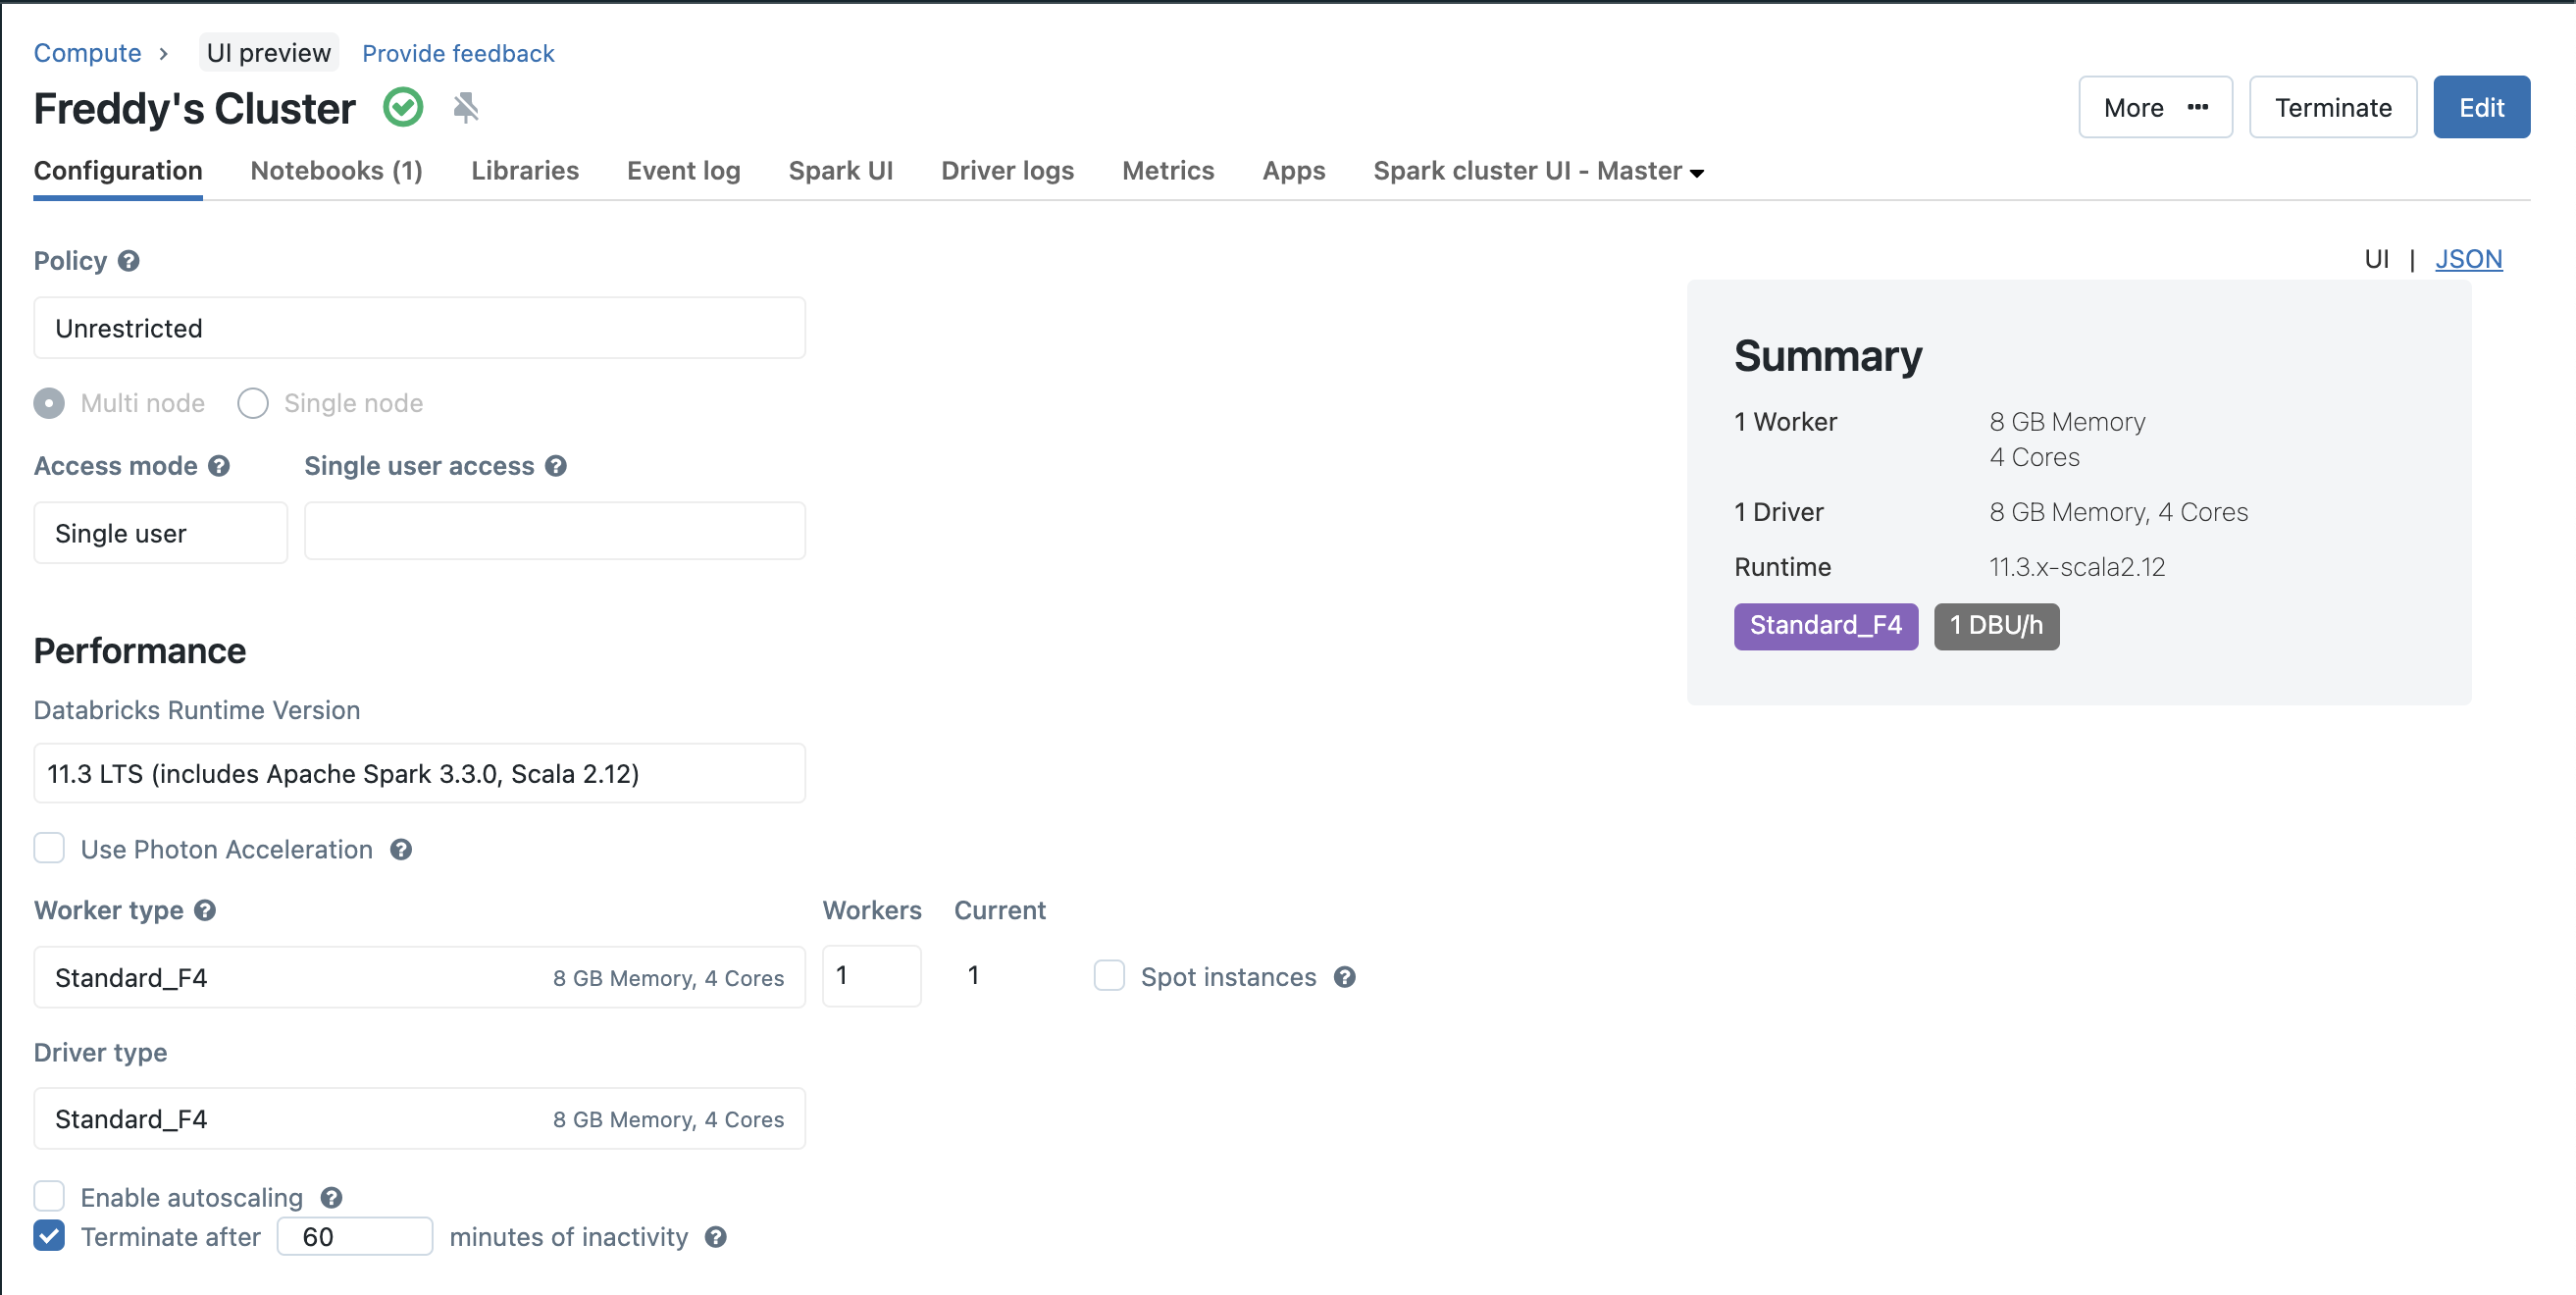
\includegraphics[width=1\textwidth]{images/databricks_configuration.png}
    \caption{Databricks Configuration}
    \label{databricks_configuration}
\end{figure}


\subsection{Apache Spark}

Apache Spark is an open-source distributed computing framework designed for processing and analyzing large-scale datasets in a highly efficient and parallel manner.
It provides a unified platform that supports various data processing tasks, including batch processing, real-time streaming, machine learning, and graph processing.
Spark's core abstraction is a resilient distributed dataset (RDD), which allows data to be distributed across multiple nodes in a cluster, enabling data processing operations to be executed in parallel \autocite{apacheSpark}.

Databricks leverages Apache Spark as its underlying engine to offer a powerful and scalable data analytics platform.
By integrating Spark into its infrastructure, Databricks provides users with a seamless and interactive environment for collaborative data engineering and data science tasks.
Databricks' interactive notebooks allow data professionals to write and execute Spark-based code, making it easier to perform data manipulations, transformations, and analysis in real-time.
The platform also offers support for various programming languages such as Python, Scala, R, and SQL, providing users with flexibility and familiarity in their preferred language.

Furthermore, Databricks enhances Apache Spark by providing additional features and optimizations to improve performance and ease of use.
The platform offers auto-scaling capabilities, enabling resources to be automatically allocated and released based on the workload demand, ensuring optimal performance and cost-efficiency.
Databricks also provides built-in libraries and tools that simplify complex tasks such as machine learning and data visualization, allowing data scientists to focus on building and deploying advanced analytical models with ease.

In summary, Apache Spark forms the backbone of Databricks, enabling the platform to handle large-scale datasets efficiently and deliver a collaborative and user-friendly environment for data analysis, making it a popular choice for organizations seeking to harness the potential of big data analytics.

\begin{figure}[h]
    \centering
    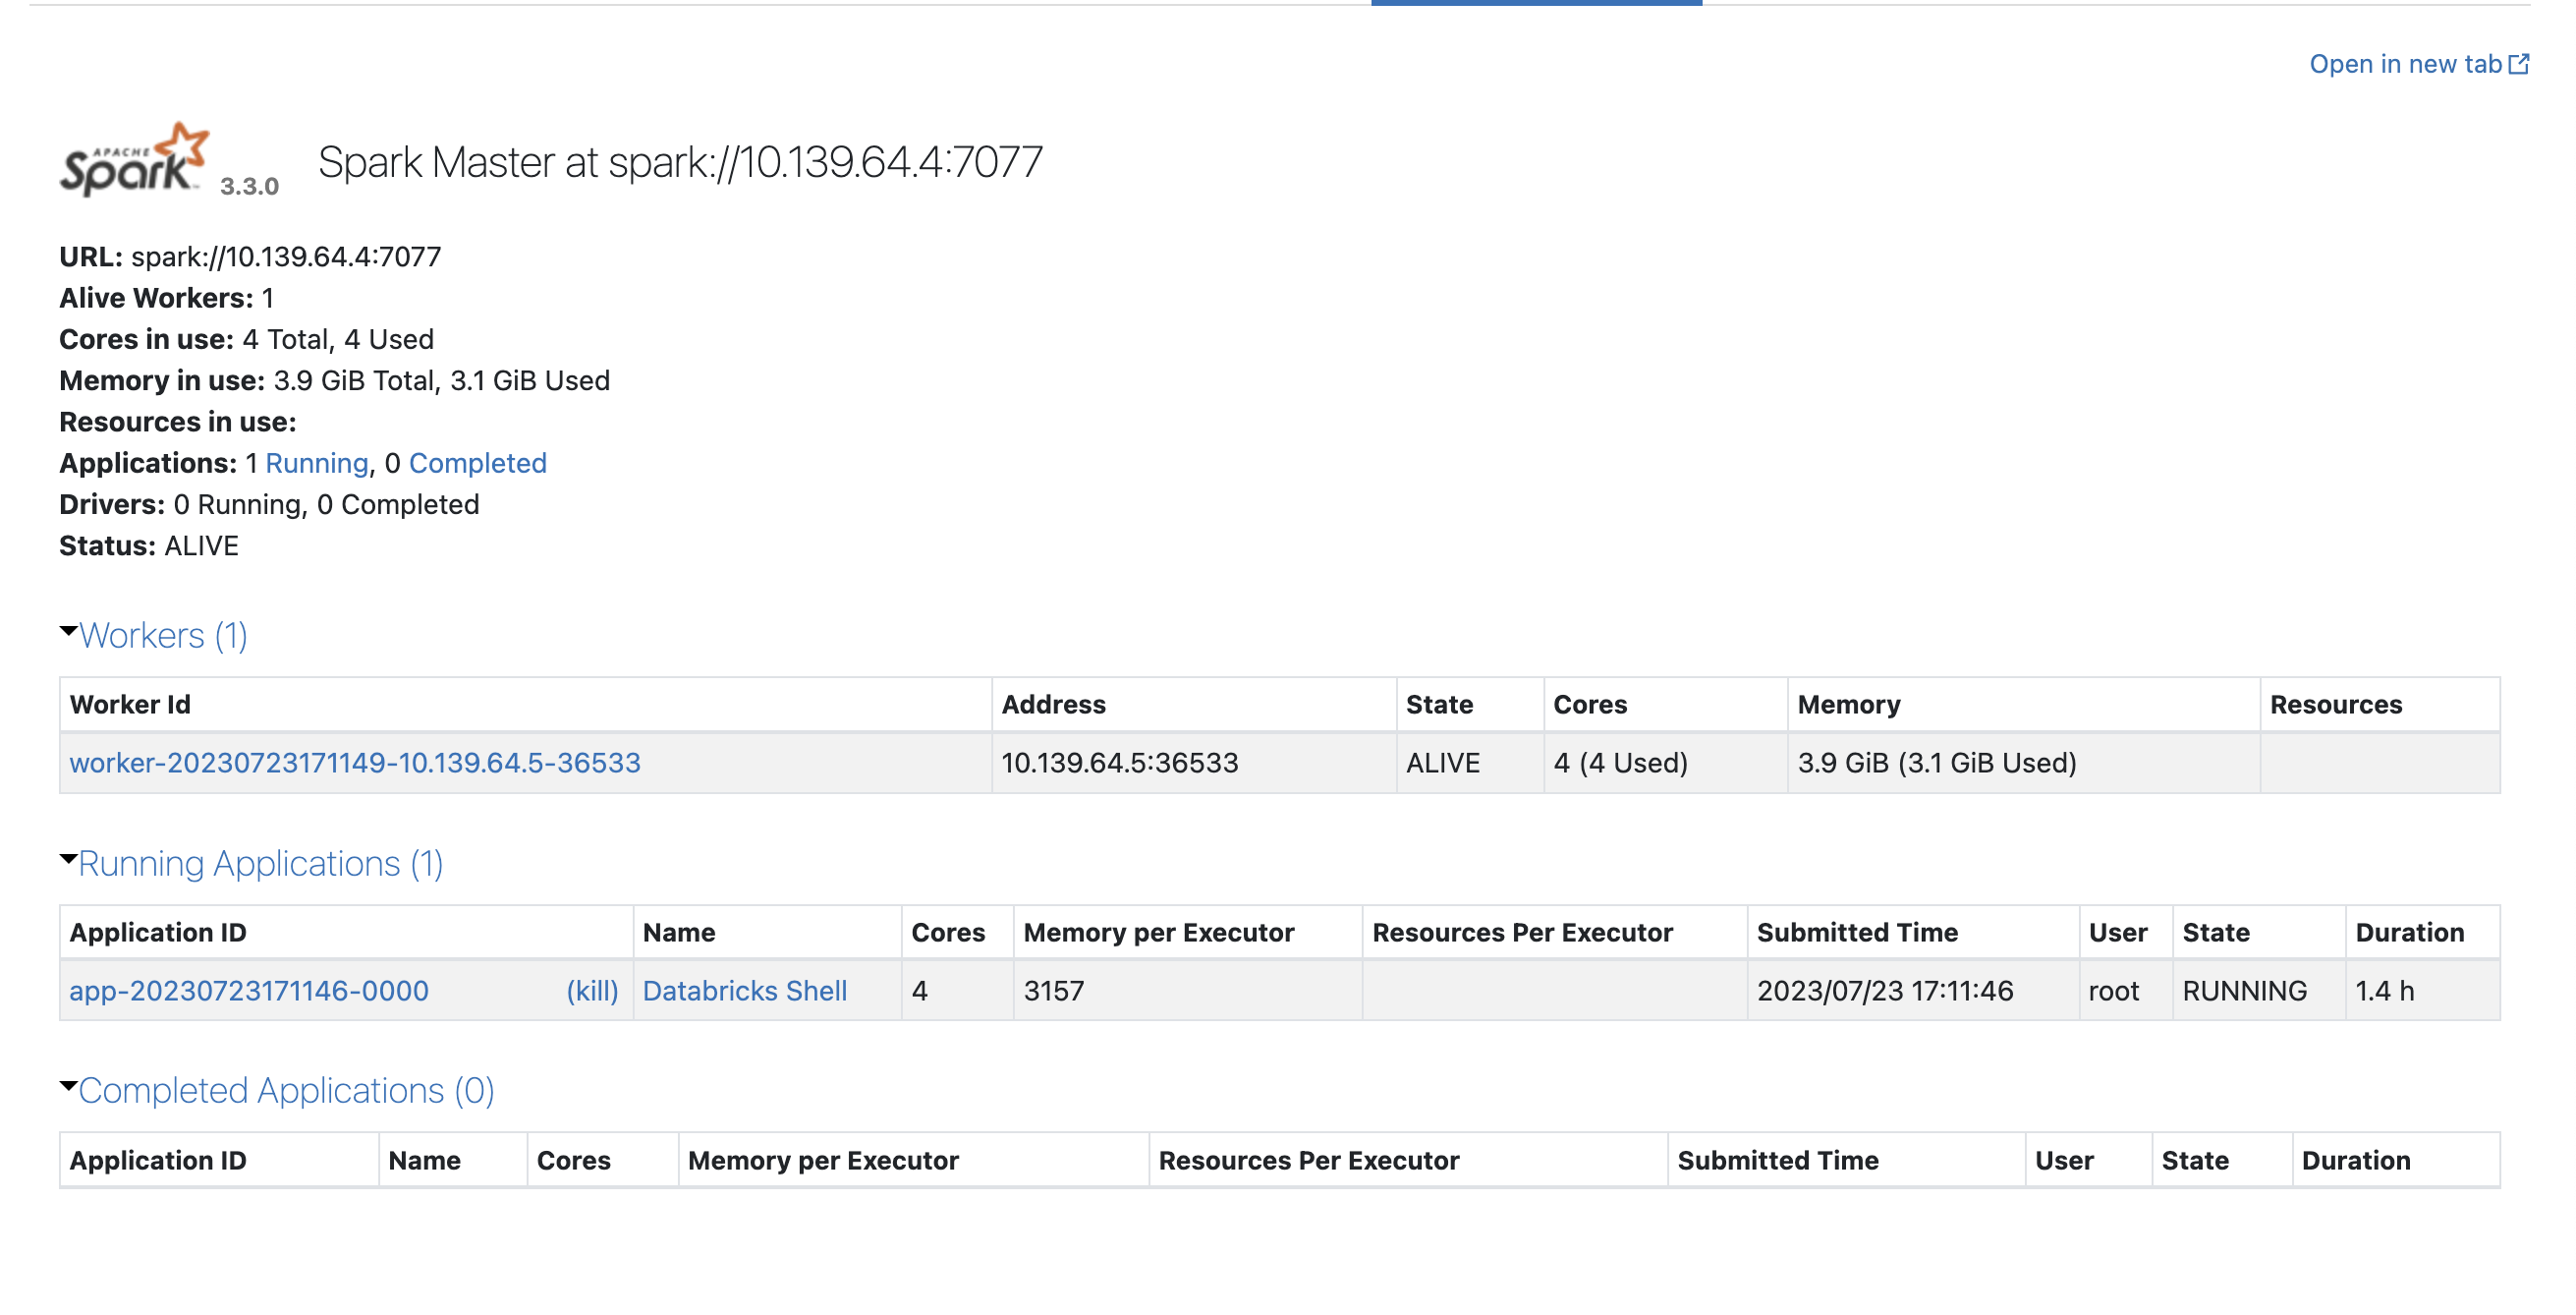
\includegraphics[width=1\textwidth]{images/spark_config.png}
    \caption{Apache Spark Configuration}
    \label{spark_config}
\end{figure}

\subsection{Astrup Fearnleys Code Emission Calculator API}

Astrup Fearnleys Code Emission Calculator API is a service that provides a simple interface for calculating the emissions of a given vessel.
The API is built on top of the Astrup Fearnleys Code Emission Calculator, It is internal tool developed to provide a simple interface for calculating the emissions of a given vessel for researchers.

It requireds the following parameters to be passed as a input:

\newpage

\begin{table}[h]
    \centering
    \begin{tabular}{|p{0.2\linewidth}|p{0.2\linewidth}|p{0.5\linewidth}|}
        \hline
        \textbf{Parameter}  & \textbf{Type} & \textbf{Description}                                                                                                          \\
        \hline
        imo                 & integer       & IMO of a ship that will require emission calculations.                                                                        \\
        \hline
        avg\_speed\_kn      & number        & The vessel's intended average sailing speed in knots on the route. Optional if duration\_h is given.                          \\
        \hline
        distance\_nm        & number        & Expected length of the voyage in Nautical Miles.                                                                              \\
        \hline
        cargo\_unit         & string        & Cargo unit used to submit cargo\_amt. Currently, the only possible value is tons. Used to calculate EEOI and transport\_work. \\
        \hline
        cargo\_amt          & number        & Amount of cargo the ship is carrying (in the given cargo\_unit). Used to calculate EEOI and transport\_work.                  \\
        \hline
        me\_fuel\_type      & string        & Fuel type to be considered for the main engine consumption for the emissions estimate. Overwriting the model assumption.      \\
        \hline
        ae\_fuel\_type      & string        & Fuel type to be considered for the auxiliary engine consumption for the emissions estimate. Overwriting the model assumption. \\
        \hline
        boiler\_fuel\_type  & string        & Fuel type to be considered for the boiler consumption for the emissions estimate. Overwriting the model assumption.           \\
        \hline
        duration\_h         & number        & Expected duration of the voyage in hours. Optional if avg\_speed\_kn is given.                                                \\
        \hline
        load\_cond          & string        & Loading condition of the vessel to be considered in the power estimation.                                                     \\
        \hline
        me\_co2\_factor     & number        & CO2 factor for the main engine fuel. Main engine fuel type must be specified.                                                 \\
        \hline
        ae\_co2\_factor     & number        & CO2 factor for the auxiliary engine fuel. Auxiliary engine fuel type must be specified.                                       \\
        \hline
        boiler\_co2\_factor & number        & CO2 factor for the boiler engine fuel. Boiler engine fuel type must be specified.                                             \\
        \hline
    \end{tabular}
    \caption{Request Parameters for Emission Calculations}
    \label{tab:request-parameters}
\end{table}

In return, it provides the JSON output in following format:


\begin{lstlisting}[language=JSON, caption=JSON output format from emission api]
    {
      "imo": 1234567,
      "avg_speed_kn": 10.045,
      "load_cond": "ballast",
      "cargo_unit": "tons",
      "cargo_amt": 544385.543,
      "me_fuel_type": "MGO",
      "ae_fuel_type": "MGO",
      "boiler_fuel_type": "MGO",
      "duration_h": 354.5,
      "me_fuel_cons_metric_metric_tons": 0.1,
      "ae_fuel_cons_metric_metric_tons": 0.1,
      "boiler_fuel_cons_metric_metric_tons": 0.1,
      "total_co2_emission_metric_tons": 0.1,
      "total_so2_emission_metric_tons": 0.1,
      "total_particulate_matter_emission_metric_tons": 0.1,
      "total_nox_emission_metric_tons": 0.1,
      "total_nmvoc_emission_metric_tons": 0.1,
      "total_ch4_emission_metric_tons": 0.1,
      "total_n2o_emission_metric_tons": 0.1,
      "total_co_emission_metric_tons": 0.1,
      "total_black_carbon_emission_metric_tons": 0.1,
      "total_organic_carbon_emission_metric_tons": 0.1,
      "transport_work": 0.1,
      "eeoi": 0.1,
      "me_co2_factor": 2.1,
      "ParamValidation": {
        "status": "OK"
      },
      "LimitMessage": {
        "message_description": "You are within your call limit"
      }
    }
    \end{lstlisting}


